
%%%%%%%%%%%%%%%%%%%%%%% file typeinst.tex %%%%%%%%%%%%%%%%%%%%%%%%%
%
% This is the LaTeX source for the instructions to authors using
% the LaTeX document class 'llncs.cls' for contributions to
% the Lecture Notes in Computer Sciences series.
% http://www.springer.com/lncs       Springer Heidelberg 2006/05/04
%
% It may be used as a template for your own input - copy it
% to a new file with a new name and use it as the basis
% for your article.
%
% NB: the document class 'llncs' has its own and detailed documentation, see
% ftp://ftp.springer.de/data/pubftp/pub/tex/latex/llncs/latex2e/llncsdoc.pdf
%
%%%%%%%%%%%%%%%%%%%%%%%%%%%%%%%%%%%%%%%%%%%%%%%%%%%%%%%%%%%%%%%%%%%


%\documentclass[runningheads,a4paper]{llncs}
\documentclass[a4paper]{./ejemplos/plantillas/llncs}

\usepackage{amssymb}
\setcounter{tocdepth}{3}
\usepackage{graphicx}

\usepackage{url}
\urldef{\mailsa}\path|{jmanuel}@bacchuss.com.ar|    
\newcommand{\keywords}[1]{\par\addvspace\baselineskip
\noindent\keywordname\enspace\ignorespaces#1}

%JMANUEL
\usepackage[utf8]{inputenc}  %con el formato de applemac no andan los acentos directos.
\usepackage[spanish]{babel}
\usepackage{enumerate}
\usepackage{}

%JMANUEL NOTAS:
% Para poner txt en itálicas: \emph{palabra}



\begin{document}

\mainmatter  % start of an individual contribution

% first the title is needed
\title{LaTeX en 10 ejemplos}

% a short form should be given in case it is too long for the running head
%\titlerunning{Lecture Notes in Computer Science: Authors' Instructions}

% the name(s) of the author(s) follow(s) next
%
% NB: Chinese authors should write their first names(s) in front of
% their surnames. This ensures that the names appear correctly in
% the running heads and the author index.
%
\author{Juan Manuel Ramon}
%
\authorrunning{Lecture Notes in Computer Science: Authors' Instructions}
% (feature abused for this document to repeat the title also on left hand pages)

% the affiliations are given next; don't give your e-mail address
% unless you accept that it will be published
\institute{Bacchuss, Investigación y Desarrollo,\\
Sarmiento 537 PB B., 2000 Rosario, Santa Fe, Argentina\\
\mailsa\\
\url{http://www.bacchuss.com.ar}}

%
% NB: a more complex sample for affiliations and the mapping to the
% corresponding authors can be found in the file "llncs.dem"
% (search for the string "\mainmatter" where a contribution starts).
% "llncs.dem" accompanies the document class "llncs.cls".
%

\toctitle{Lecture Notes in Computer Science}
\tocauthor{Authors' Instructions}
\maketitle


\begin{abstract}
Se plantea una linea de trabajo con orientación fuertemente práctica para aprender el lenguaje de procesamiento de textos LaTeX por medio del análisis de 10 ejemplos básicos que contienen la mayoría de los recursos utilizados en la generación de documentos profesionales.

Junto a este manual se distribuye un directorio (\verb+/ejemplos+) que contiene el código fuente de todos los ejemplos tratados, y tres directorios extra (\verb+/plantillas, /img, y /capítulos+) con todos los recursos necesarios para realizar las prácticas.

\end{abstract}



\section{Introducción}

La creación de documentos en LaTeX es relativamente simple siempre que se cumpla con algunos pasos que en general tienen que ver con:

\begin{enumerate}[a.]
\setlength\itemindent{10pt} \item {\bfseries Edición base:} creación del contenido (en un editor de texto cualquiera, con corrección ortográfica finalizada, ej:.txt).
\setlength\itemindent{10pt} \item {\bfseries Preparación del documento LaTeX:} creación de archivo fuente (se crea un archivo plano con los encabezados y contenidos con extensión .tex).
\setlength\itemindent{10pt} \item {\bfseries Compilación y salida DVI:} creación del documento visualizable DVI (.dvi) a partir del .tex.
\setlength\itemindent{10pt} \item {\bfseries Creación de salida PDF:} creación del documento visualizable PDF (.pdf) a partir del .dvi
\end{enumerate}

En general, salvo funcionalidades específicas, la secuencia de comandos para la compilación de un documento simple es la liguiente (desde .tex hasta .pdf):

\begin{verbatim}
# látex ejemplo.tex	(genera salida "ejemplo.dvi")
# dvipdf ejemplo.dvi	(genera salida "ejemplo.pdf")
\end{verbatim}


\section{Ejemplo 1: Creación de un documento base}
Todo documento LaTeX posee dos componentes fundamentales:

\begin{enumerate}[a.]
\setlength\itemindent{10pt} \item {\bfseries Encabezados y directivas}
\setlength\itemindent{10pt} \item {\bfseries Contenidos}
\end{enumerate}

Los encabezados y directivas permiten dar formato al documento, con una gran cantidad de opciones para cuestiones tales como lenguajes, manejo de imágenes, ecuaciones matemáticas, notas al pié y encabezados, numeración, etc.
\newline
A continuación se analiza un documento básico, sin ningún tipo de formato ni funcionalidad extra, que ni siquiera es capaz de procesar los caracteres del idioma Español:

\begin{verbatim}
# vi ejemplo1.tex
\documentclass{article}
\begin{document}
Este es el texto que queremos hacer en formato Latex para que 
se pueda hacer una publicación seria.
Saludos.
Juan Manuel.
NOTA: en este doc no se ven los acentos ni las ennnnes.
\end{document}
\end{verbatim}


\section{Ejemplo 2: Documento en Español con código fuente}

Para que el intérprete LaTeX pueda procesar los caracteres especiales del Español, ademas de configurar correctamente la herramienta (ver Sección 12), será necesario incluir algunas librerías extra en el encabezado:

\begin{enumerate}[a.]
\setlength\itemindent{10pt} \item {\bfseries}\verb+\usepackage[utf8]{inputenc} +
\setlength\itemindent{10pt} \item {\bfseries}\verb+\usepackage[spanish]{babel} + 
\end{enumerate}


El siguiente código LaTeX no posee ningún formato especial, pero es capaz de procesar los caracteres del idioma Español:

\begin{verbatim}
# vi ejemplo2.tex
\documentclass[a4paper{article}
%JMANUEL
\usepackage[utf8]{inputenc}  
\usepackage[spanish]{babel}

\begin{document}
Este es el texto que queremos hacer en formato Latex ...

A continuación se muestra como introducir código fuente:
\begin{verbatim}
  	<?php
	$passwordHash = sha1($_POST['password']);
	$sql = 'INSERT INTO user (user,passHash) VALUES (?,?)';
	$result = $db->query($sql, array($_POST['user'], $passHash));?>
	\end{document}

\end{verbatim}

Además, puede verse que para el código fuente se han utilizado las sentencias \verb+ \begin{verbatim} y \end{verbatim}+ que permiten interpretar la entrada como texto en typewriter, e ignora comando LaTeX en su interior.


\section{Ejemplo 3: Un documento con imágenes}

La inclusión de imágenes en un documento Latex debe atender dos cuestiones:

\begin{enumerate}[a.]
\setlength\itemindent{10pt} \item {\bfseries Formato de la imagen:} las imágenes deben ser transportadas a formato '.eps'. EPS (Encapsulated PostScript \cite{b1}) es el formato adecuado para evitar conflictos en los casos que se deseen generar salidas PS o PDF.
\setlength\itemindent{10pt} \item {\bfseries Formato del documento:} tamaño, posición, transparencia, texto asociados, se controlan todos por medio de las directivas Latex. Las directivas de posición son 'here'(h), 'top'(t), 'bottom'(b) y 'whole-page'p. Una opción muy común para tener control absoluto de la posición de la imágen en el texto es especificar la directiva de tipo \verb+\begin{figure}[!htb]+ \cite{b2}\cite{b3}.
\end{enumerate}

Para transformar las imágenes a formato EPS: \newline 
\verb+ #convert img1.png img1.eps +
\newline \newline 
además se debe incluir la directiva Latex: \newline
\verb+ \usepackage{graphicx} +

\begin{verbatim}
# vi ejemplo3.tex
\documentclass{article}
%JMANUEL
\usepackage{graphicx}

\begin{document}
En la Figura 1 puede verse un esquema: \newline
\begin{figure}[!htb]\centering
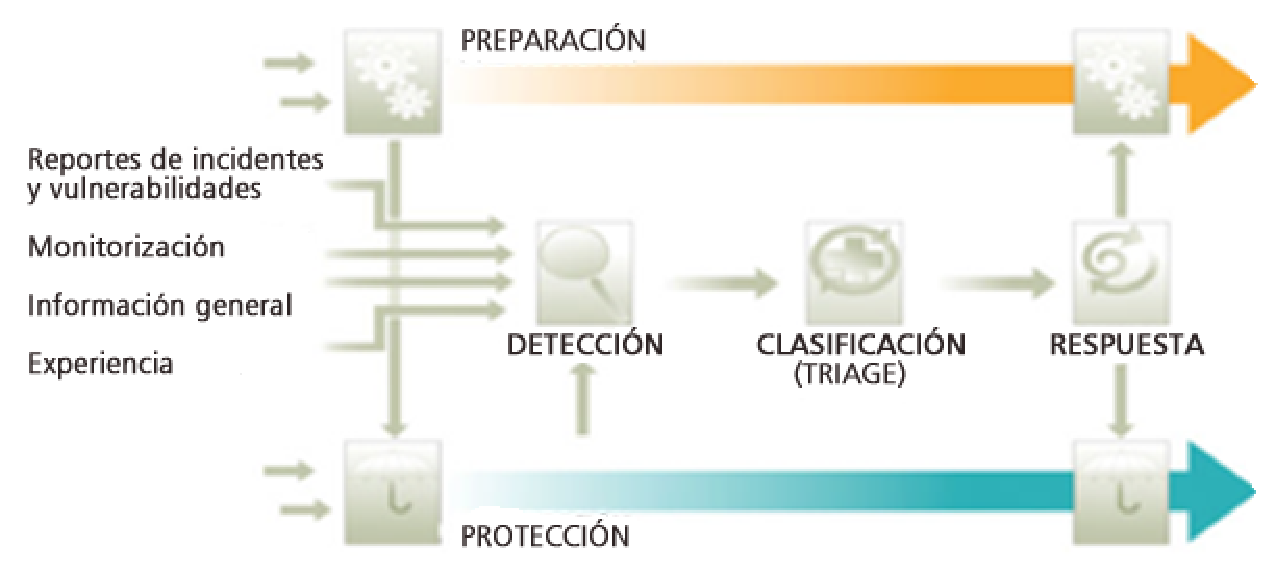
\includegraphics[scale=0.4]{./img/1-gis}
\caption{Este sería el texto de la gráfica}\end{figure}
\end{document}
\end{verbatim}


\section{Ejemplo 4: Un documento compuesto}

La generación de un único documento a partir de varios capítulos editados por separado es muy simple gracias a las directiva \verb+\include+ de LaTeX. El único cuidado que debe tenerse es mantener coherencia entre las directivas de formato en cada una de las partes que conformaran el documento final.

En el archivo raíz se hace referencia a todos los fuentes parte del documento como puede verse en el siguiente ejemplo:

\begin{verbatim}
# vi ejemplo4.tex
\documentclass{article}
%JMANUEL
\usepackage[utf8]{inputenc}  
\usepackage[spanish]{babel}
\usepackage{graphicx}

\begin{document}
Capitulo1: \newline
La generación de un único documento a partir de varios capítulos editados por separado es muy simple gracias a las directiva include de Latex. El único cuidado que debe tenerse es mantener coherencia entre las directivas de formato en cada una de las partes que conformaran el documento final.

\include{./capitulos/capitulo2}
\end{document}
\end{verbatim}

Ahora, a modo informativo se muestra el contenido del\verb+ capitulo1.tex+:

\begin{verbatim}
Capitulo1:\newline
La generación de un único documento a partir de varios capítulos 
editados por separado es muy simple gracias a las directiva include 
de Latex. El único cuidado que debe tenerse es mantener coherencia 
entre las directivas de formato en cada una de las partes que 
conformaran el documento final.
\end{verbatim}


\section{Ejemplo 5: Referencias bibliográficas en LaTeX}

Existen dos formas de generar bibliografías en documentos, una simple por medio de directivas LaTeX que puede ser utilizada para artículos cortos en las que no se utilizan gran cantidad de referencias, y otra mas compleja para tesis o libros en cuyo caso se utiliza una herramienta suplementaria conocida como "bibTex"\cite{b4}.

\subsection{Referencias simples en LaTeX}

A continuación se presenta un ejemplo del método simple, que es el mismo utilizado en el presente documento, en el que las referencias están incluídas en el mismo cuerpo del documento y donde no hace falta la ejecución de comando especiales de LaTeX para el procesamiento de las mismas.

\begin{verbatim}
# vi ejemplo5-simple.tex
\documentclass{article}
%JMANUEL
\usepackage[utf8]{inputenc}  
\usepackage[spanish]{babel}

\begin{document}
Existen dos formas de generar bibliografías en documentos 
una simple \cite{simple} por medio de... y otra mas 
compleja \cite{bibtex} para Tesis o Libros en cuyo caso 
se utiliza una herramienta "bibTex" .

\begin{thebibliography}{1}
  \bibitem{simple}Juan Dower {\em Compilado 479.}  1991.
  \bibitem{bibtex}Japan Reader {\em Japon 1945} 1973: N.Y. 
\end{thebibliography}
\end{document}
\end{verbatim}




\subsection{Referencias con Bibtex}

BibTeX es una herramienta para dar formato a listas de referencias que se utiliza habitualmente con el sistema de preparación de documentos LaTeX, facilita la realización de citas bibliográficas de un modo consistente mediante la separación de la información bibliográfica de la presentación de esta información. BibTeX usa un formato de archivo (\verb+.bib+) basado en texto e independiente del estilo para definir listas de elementos bibliográficos, como artículos, libros, tesis. \newline

Supóngase que se está trabajando sobre un artículo (\verb+ejemplo5-bibtex.tex+) y que se desea agregar las referencia utilizando el formato bibtex. Lo primero que deberá hacerse es crear un archivo de bibliografía (.bib) al cual se llamará \verb+ejemplo5-bibtex.bib+ el cuál incluirá todas las referencias en base al siguiente formato general:

\begin{verbatim}
@BOOK{<alguna abreviatura que se genere para la referencia>,
	    AUTHOR = "autor",
	    TITLE = "título del trabajo",
	    PUBLISHER = {Compañía editora},
	    ADDRESS = {lugar de publicación},
	    YEAR = año de publicación}
\end{verbatim}

Una vez generado el archivo \verb+.bib+, para refenciar en el texto a la entrada deseada de la bibliografía se deberá recurrir a la directiva \verb+"\cite"+. Finalmente, en la parte del documento principal (artículo) en la cuál se desea introducir la bibliografía se deberán especificar las directivas propias de bibtex:

\begin{verbatim}
\bibliography{ejemplo5-bibtex}
\bibliographystyle{plain}
\end{verbatim}

Nota: si se tienen referencias que no se citan explícitamente en el texto, pero que a pesar de esto se desea incluirlas en la lista de referencias, entonces deberá utilizarse la directiva \verb+\nocite {baz,fuzz,bong}+ en el documento \verb+ejemplo5-bibtex.tex+.\newline

Una vez generados los archivos \verb+.tex+ y \verb+.bib+, se deberá ejecutar la siguiente secuencia general de comandos:

\begin{verbatim}
# latex ejemplo5-bibtex.tex   	(genera .aux usado por bibtex)
# bibtex ejemplo5-bibtex  		(genera un archivo de salida .bbl)
# latex ejemplo5-bibtex.tex		(inserta entradas de .bbl en texto)
# latex ejemplo5-bibtex.tex		(refina las referencias en el texto)
\end{verbatim}

A continuación se presenta un ejemplo del método utilizando "bibtex".


\begin{verbatim}
# vi ejemplo5-bibtex.tex
\documentclass{article}
%JMANUEL
\usepackage[utf8]{inputenc}  
\usepackage[spanish]{babel}

\begin{document}
La artista y activista por la paz Yoko Ono \cite{primero}
se unió al llamamiento para la liberación de las tres integrantes 
de la banda punk rusa Pussy Riot \cite{segundo}, alabando 
su postura \cite[p. 2]{tercero} en favor de la libertad de 
expresión después de ser condenadas a dos años de prisión por 
organizar "una oración punk" en la principal catedral de Moscú.

\bibliography{ejemplo5-bibtex}
\bibliographystyle{plain}
\end{document}
\end{verbatim}


En este archivo, la directiva \verb+\bibliography{ejemplo5-bibtex}+ implica que el nombre del archivo de base de datos (.bbl) será \verb+"ejemplo5-bibtex"+, mientras que  \verb+\bibliographystyle{plain}+ es la directiva que establece el formato de las referencias. Mientras que la opción \verb+"plan"+ muestra solo el número de referencia entre corchetes, opciones como \verb+"abbrv"+ muestran el apellido resumido de los autores, \verb+"alfa"+ muestra letras en lugar de números, e \verb+"ieeetr"+ ordena las referencias por orden de aparición en lugar de en orden alfabético.

\begin{verbatim}
# vi ejemplo5-bibtex.bib
@book{primero,
   title = "A Handbook for Scholars",
   author = "Aberdeen, Mary-Claire",
   publisher = "Knopf",
   year = "1979"
   }

@BOOK{segundo,
	    AUTHOR = "Baberdeen, R. M.",
	    TITLE = "Foo Bar Baz",
	    PUBLISHER = {MIT Press},
	    ADDRESS = {Cambridge, MA},
	    YEAR = 1989}

@ARTICLE{tercero,
   AUTHOR  = {Caberdeen, R. W.},
   TITLE   = {Interannual Variability of {M}ars},  
   YEAR    = {1993},
   JOURNAL = jgr,
   VOLUME  = {98},
   NUMBER  = {E2},
   PAGES   = {3247--3259}
}
\end{verbatim}



\section{Ejemplo 6: Capítulos, secciones, y tabla de contenidos}

Será conveniente presentar el estudio de capítulos, secciones y tablas de contenido (toc) en base a dos formatos esenciales de documentos en LaTeX\cite{b5}:

\begin{enumerate}[a.]
\setlength\itemindent{10pt} \item {\bfseries Artículos:} textos relativamebte cortos en los que el índice va junto al título del documento.
\setlength\itemindent{10pt} \item {\bfseries Libros:}  textos extensos en los que el índice va separado de los datos básicos del documento como título, autores, fechas, etc.
\end{enumerate}


\subsection{Artículos en Latex}

Los artículos se generan a partir de las directivas: 
\begin{enumerate}[-]
\setlength\itemindent{10pt} \item {\bfseries }\verb+\section{Nombre}+, 
\setlength\itemindent{10pt} \item {\bfseries }\verb+\subsection{Nombre}+ y 
\setlength\itemindent{10pt} \item {\bfseries }\verb+\subsubsection{Nombre}+. 
\end{enumerate}

No es necesario definir la numeración de secciones y páginas ya que LaTeX la mantiene de manera automática. Este es un ejemplo sumamente sintético de algunos de los elementos fundamentales necesarios para la generación de un artículo en LaTeX. Entre estos se presenta el uso de:


\begin{enumerate}[a.]
\setlength\itemindent{10pt} \item {\bfseries \verb+\documentclass{article}+}
\setlength\itemindent{10pt} \item {\bfseries \verb+\title{Título del artículo}+}
\setlength\itemindent{10pt} \item {\bfseries \verb+\author{Nombre del autor}+}
\setlength\itemindent{10pt} \item {\bfseries \verb+\date{Fecha de realización}+}
\setlength\itemindent{10pt} \item {\bfseries \verb+\maketitle+}
\setlength\itemindent{10pt} \item {\bfseries \verb+\tableofcontents+}
\end{enumerate}

A continuación se presenta un breve ejemplo:\newline\newline

\begin{verbatim}
# vi ejemplo6-articulo.tex
\documentclass{article}
%JMANUEL
\usepackage[utf8]{inputenc} 
\usepackage[spanish]{babel}

\begin{document}
\title{Como estructurar un artículo en LaTeX}
\author{Juan Manuel Ramon}
\date{Setiembre de 2012}
\maketitle
\begin{abstract}
Esta es la sección que contiene el abstracto del documento...
\end{abstract}
\newpage
% Para agregar el índice, puede ser omitido.
\tableofcontents
\newpage

\section{Introduccción}
Esta es la sección de introcucción...

\section[Estructura]{Un análisis de lo estructuralmente 
significativo para el modelo}
Esta es la sección de estructuras...
\subsection{Primera subsección}
Contenido de la primera subsección...
\subsubsection{Primera subsubsección}
Contenido de la primera subsubsección...
\subsection{Segunda subsección}
Contenido de la segunda subsección...

\end{document}
\end{verbatim}


Nota: es interesante ver en la segunda sección, que para que los títulos largos no afecten la tabla de contenidos es posible modificar su comportamiento.


\subsection{Libros en Latex}

Este es un ejemplo sumamente sintético de algunos de los elementos fundamentales necesarios para la generación de un libro en LaTeX. Entre estos se presenta el uso de:

\begin{enumerate}[ a. ]
\setlength\itemindent{10pt} \item {\bfseries \verb+\documentclass{book}+}
\setlength\itemindent{10pt} \item {\bfseries \verb+\frontmatter+}
\setlength\itemindent{10pt} \item {\bfseries \verb+\appendix+}
\end{enumerate}

\begin{verbatim}
# vi ejemplo6-libro.tex
\documentclass{book}
%JMANUEL
\usepackage[utf8]{inputenc}  
\usepackage[spanish]{babel}

\begin{document}
\title{Como estructurar un libro en LaTeX}
\author{Juan Manuel Ramon}
\date{Setiembre de 2012}
\maketitle
\frontmatter

% Para agregar el índice, puede ser omitido.
\tableofcontents

\chapter{Introducción}
Aquí escribo la introducción. Cada párrafo se separa con una línea 
en blanco.
\mainmatter
 
\chapter{Primero lo primero}
Puedo hacer que el texto vaya en cursiva \emph{texto en cursiva}. 

\chapter{Segundo le sigue}
Las notas a  pie se hacen con...

\section{Introduccción}
Texto de la sección de introducción...

\subsection{Primera subsección}
Texto de la priimera subsección de estructuras...

\subsection{Segunda subsección}
Texto de la segunda subsección de estructuras...

\appendix
\chapter{Primer apéndice}
Texto del priimer apéndice...
\chapter{Segundo apéndice}
Texto del segundo apéndice...
\backmatter

\end{document}
\end{verbatim}


Los apéndices por defecto se numeran diferente en LaTeX, en lugar de números se utilizan letras imprenta mayúsculas. La directiva \verb+\appendix+ debe ser utilizada una única vez para todos los apéndices.\newline

Nota: ver que tanto en la sección de artículos y de libros se han utilizado modificadores para la presentación de listas de enumeración, laterando tanto los índices como las sangrías de cada elemento por medio de las facilidades que entrega tanto LaTeX como el paquete \verb+\usepackage{enumerate}+.



\section{Ejemplo 7: Un documento con indice de términos}

Un índice de términos (índice) es una lista ordenada alfabéticamente de palabras y expresiones muy útil para ser utilizado en libros. La creación de índices hace uso del paquete \verb+\usepackage{makeidx}+ de LaTeX, y del comando \verb+'makeindex'+ \cite{b6}. Para los casos en que resulte útil, existen diferentes opciones de índices anidados. Para aplicar un índice será necesario utilizar un paquete especial y las directivas enunciadas a continuación:

\begin{enumerate}[a.]
\setlength\itemindent{10pt} \item {\bfseries \verb+\usepackage{makeidx}+}
\setlength\itemindent{10pt} \item {\bfseries \verb+\makeindex+}
\setlength\itemindent{10pt} \item {\bfseries \verb+\printindex+}
\end{enumerate}

El primer paso consiste en aplicar látex sobre el archivo para que la herramienta genere el archivo de índices (.idx), el cuál será tomado nuevamente por látex para generar los enlaces a cada término. La secuencia para compilar un documento LaTeX con índice es:

\begin{verbatim}
# latex ejemplo7.tex
# makeindex ejemplo7.idx
# latex ejemplo7.tex
# dvipdf ejemplo7.dvi
\end{verbatim}

A continuación se presenta un ejemplo con algunas variantes de uso:

\begin{verbatim}
# vi ejemplo7.tex
\documentclass{article}
%JMANUEL
\usepackage[utf8]{inputenc}
\usepackage[spanish]{babel}
\usepackage{makeidx}

\title{Mi primer índice}
\makeindex

\begin{document}
\maketitle
Hola mundo\index{mundo}...
\newpage
Este es nuestro lugar en el mundo\index{mundo}...
algo totalmente terrenal\index{mundo!terrenal}...
\newpage
Este es nuestro lugar en el mundo\index{mundo}...
algo totalmente terrenal\index{mundo!terrenal}... 
y totalmente mágico\index{fantasía!mágico}.

\printindex
\end{document}
\end{verbatim}



\section{Ejemplo 8: Un documento con glosario de términos}

En general, en documentos técnicos se hace uso de términos o acrónimos que pueden resultar desconocidos para el lector. Para hacer mas accesibles los documentos se utiliza el glosario. A tal fin se utiliza el paquete \verb+"glossaries"+ de LaTeX, que sirve para incluir diversos glosarios, acrónimos y símbolos.\newline

Para generar un glosario se debe\cite{b7}:

\begin{enumerate}[a.]
\setlength\itemindent{10pt} \item {\bfseries} Definir \verb+\usepackage{glossaries}+ y \verb+\makeglossaries+ en el preámbulo del documento (después de \verb+\usepackage{hyperref}+ si existe).
\setlength\itemindent{10pt} \item {\bfseries} Definir las entradas \verb+\newglossaryentry+ y \verb+\newacronym+ para glosarios y acrónimos en el preámbulo (recomendado), o antes de su utilización.
\setlength\itemindent{10pt} \item {\bfseries} Finalmente añadir \verb+\printglossaries+ en el lugar donde se desee imprimir el glosario, y de existir la lista de acrónimos.
\end{enumerate}

Luego se deben ejecutar los siguientes comandos:

\begin{verbatim}
# latex ejemplo8-base.tex
# makeglossaries ejemplo8-base
# latex ejemplo8-base.tex
# dvipdf ejemplo8-base.dvi
\end{verbatim}


A continuación se presenta un ejemplo en el que se utilizan dos archivos auxiliares (\verb+.tex+) para definir el glosario y la lista de acrónimos por separado y así tener mayor orden y control.

\begin{verbatim}
# vi ejemplo8-base.tex
\documentclass{article}
%JMANUEL
\usepackage[utf8]{inputenc}  
\usepackage[spanish]{babel}
\usepackage[spanish]{translator}

\usepackage[acronym]{glossaries}
\makeglossaries
\newglossaryentry{computadora}
{
  name=computadora,
  description={se debe considerar que esencialmente es un aparato que hay en muchas casas que sirve para programar y divertirse.}
}

\newglossaryentry{lavarropas}
{
  name=lavarropas,
  description={se debe considerar que esencialmente es un aparato que hay en muchas casas que sirve para lavar la ropa.}
}

\newacronym{pdf}{PDF}{Portable Document Format}
\newacronym{ids}{IDS}{Intrusion Detection Systems}



\title{Mi primer doc con glosario y acrónimos}

\begin{document}
\maketitle
La \gls{computadora} no tiene nada que ver con el \gls{ids} 
y mucho menos con el \gls{lavarropas}.
\newpage
Toda la documentación de los \gls{ids} deberá estar en 
formato \gls{pdf}.
\newpage
% definición del glosario
\printglossary[type=main]
\newpage
% definición de acrónimos
\printglossary[type=\acronymtype]
\end{document}
\end{verbatim}


Además debe definirse la listas de glosario:

\begin{verbatim}
# vi ejemplo8-glosario.tex
\newglossaryentry{computadora}
{
  name=computadora,
  description={se debe considerar que esencialmente es un 
  aparato que hay en muchas casas que sirve para programar 
  y divertirse.}
}
\newglossaryentry{lavarropas}
{
  name=lavarropas,
  description={se debe considerar que esencialmente es un 
  aparato que hay en muchas casas que sirve para lavar 
  la ropa.}
}
\end{verbatim}


y la de acrónimos:

\begin{verbatim}
# vi ejemplo8-acronimos.tex
\newacronym{pdf}{PDF}{Portable Document Format}
\newacronym{ids}{IDS}{Intrusion Detection Systems}
\end{verbatim}


En el archivo de salida debe observarse el comportamiento de los acrónimos ya que la primera vez que estos son reverenciados se incluye su nombre completo, en referencias sucesivas solo sus siglas (Por ejemplo: la primera vez se muestra Intrusion Detection Systems (IDS), y luego solo IDS).\newline

La presentación de los términos puede ser controlada mediante opciones de referencia como por ejemplo\cite{b8}\cite{b9}:

\begin{enumerate}[a.]
\setlength\itemindent{10pt} \item {\bfseries \verb+\gls{etiqueta}:+}  uso tradicional, forma singular en minúscula.
\setlength\itemindent{10pt} \item {\bfseries \verb+\glspl{etiqueta}:+}  referencia al plural definido para un término (si es que no finaliza con s, ej: maiz-maices).
\setlength\itemindent{10pt} \item {\bfseries \verb+\Gls{etiqueta}:+}  uso tradicional, forma singular con la primera letra en mayúscula.
\setlength\itemindent{10pt} \item {\bfseries \verb+\Glspl{etiqueta}:+}  referencia al plural definido para un término, pero con la primera letra en mayúscula.
\setlength\itemindent{10pt} \item {\bfseries \verb+\glslink{<etiqueta>}{<texto alternativo>}:+}  genera un enlace como en el resto de los casos, pero permite una definición alternativa.
\end{enumerate}


Para el caso particular de acrónimos, deberá considerarse que su comportamiento es un poco diferente al de los glosarios. En su primera utilización, al referenciar un acrónimo se mostrara el texto \verb+"<full> (<abbrv>)"+, mientras que en subsecuentes usos del mismo solo se mostrará \verb+"(<abbrv>)"+.

\begin{enumerate}[a.]
\setlength\itemindent{10pt} \item {\bfseries \verb+\glsreset{<etiqueta>}:+}  reseteo del uso del acrónimo referenciado.
\setlength\itemindent{10pt} \item {\bfseries \verb+\glsresetall:+} respeta todos los acrónimos.
\end{enumerate}


Para incluir un glosario y una lista de acrónimos en la lista de contenidos (TOC) del documento se deben utilizar las siguientes directivas en el encabezado del documento:

\begin{enumerate}[i.]
\setlength\itemindent{10pt} \item {\bfseries }\verb+\usepackage[toc,acronym]{glossaries}+
\setlength\itemindent{10pt} \item {\bfseries }\verb+\makeglossaries+
\end{enumerate}

El ejemplo desarrollado (\verb+"ejemplo8-tocglos.tex"+) se ha utiliza como base el libro del capítulo 6 (\verb+"ejemplo6-libro.tex"+).


\section{Ejemplo 9: Ecuaciones en Latex}

Escribir ecuaciones fué una de las principales motivaciones de Donald Knuth al desarrollar LaTeX. La potencia que alcanzó la herramienta para tal fin la hizo muy popular en el ambiente científico para la generación de documentos\cite{b10}.\newline

Para documentos que requieran una serie de fórmulas simples, las herramientas incluídas por defecto en LaTeX serán suficiente, ahora si se requiere la edición de documentos con muchas fórmulas, con complejidad media o alta, entonces deberá recurrirse al paquete \verb+"amsmath"+ \cite{b11}. Para este último caso puede utilizarse como opción al paquete \verb+"mathtools"+\cite{b12} que agrega funciones y flexibiliza a \verb+amsmath+.\newline

 Según sea el caso, deberá incluírse el paquete correspondiente en el encabezado del documento mediante las directivas:
 
\begin{enumerate}[i.]
\setlength\itemindent{10pt} \item {\bfseries } \verb+\usepackage{amsmath}+, ó
\setlength\itemindent{10pt} \item {\bfseries } \verb+\usepackage{mathtools}+.
\end{enumerate}

Nota: el paquete \verb+mathtools+ carga al paquete \verb+amsmath+ de manera automática.\newline

Siempre que se definían ecuaciones, LaTeX debe ser informado ya que la forma de interpretar a la entrada difiere del modo convencional de texto. Para esto existen dos formas que tienen que ver con la manera en que se introducirá la expresión en el documento, cada una de las cuales obedecerá a la configuración particular del ambiente:

\begin{enumerate}[a.]
\setlength\itemindent{10pt} \item {\bfseries Ecuación en linea con el texto (Text):} se utilizan las directivas\newline \verb+\begin{math}...\end{math}+, o la forma corta \verb+"\(…\)"+. \newline Ejemplo: "la expresión 2x+2=4 deberá ser contemplada…"). 
\setlength\itemindent{10pt} \item {\bfseries Ecuación separada del texto (Displayed):} se utilizan las directivas:\newline 
   \verb+\begin{displaymath}...\end{displaymath}+, o la forma corta \verb+"\[…\]"+. \newline
   Opcionalmente puede utilizarse \verb+\begin{equation*}...\end{equation*}+.
\end{enumerate}   


Independientemente del formato de introducción de la fórmula, se deben conocer los diferentes símbolos matemáticos, su significado, y su formato de salida (producto). A continuación se presenta una lista de recursos utilizados para ecuaciones en LaTeX \cite{b10}\cite{b13}:

\begin{enumerate}[a.]
\setlength\itemindent{10pt} \item {\bfseries} Símbolos
\setlength\itemindent{10pt} \item {\bfseries} Letras Griegas
\setlength\itemindent{10pt} \item {\bfseries} Operadores
\setlength\itemindent{10pt} \item {\bfseries} Potencias e índices
\setlength\itemindent{10pt} \item {\bfseries} Fracciones y binómios
\setlength\itemindent{10pt} \item {\bfseries} Fracciones y binómios
\setlength\itemindent{10pt} \item {\bfseries} Raíces
\setlength\itemindent{10pt} \item {\bfseries} Sumas e integrales
\setlength\itemindent{10pt} \item {\bfseries} Delimitadores como corchetes, paréntesis y otros
\setlength\itemindent{10pt} \item {\bfseries} Matrices y vectores
\setlength\itemindent{10pt} \item {\bfseries} Texto en la ecuaciones
\setlength\itemindent{10pt} \item {\bfseries} Formatos de los símbolos
\setlength\itemindent{10pt} \item {\bfseries} Símbolos de suma y resta
\setlength\itemindent{10pt} \item {\bfseries} Control de espacio horizontal
\setlength\itemindent{10pt} \item {\bfseries} Lenguajes avanzados: amsmath y mathtool
\end{enumerate}


El siguiente ejemplo muestra el uso de los dos tipos de definición:

\begin{verbatim}
# vi ejemplo9.tex
\documentclass{article}
%JMANUEL
\usepackage[utf8]{inputenc} 
\usepackage[spanish]{babel}
\usepackage{mathtools}

\begin{document}
Mi primera ecuación en LaTeX.

A. Formato en línea ("Text")
A la expresión 
\( x \leq 21 \) 
, si se la instacia con 19 da bien.
\newline

B. Formato separado ("Displayed")
\newline
La siguiente expresión:
\[
 \forall x \in X, \quad \exists y \leq \epsilon
\]
puede ser connsiderada por diversos motivos como un...
\newline

Una serie:
\[
 {n! \over k!(n-k)!} = {n \choose k}
\]

Una matríz:
\[
 A_{m,n} =
 \begin{pmatrix}
  a_{1,1} & a_{1,2} & \cdots & a_{1,n} \\
  a_{2,1} & a_{2,2} & \cdots & a_{2,n} \\
  \vdots  & \vdots  & \ddots & \vdots  \\
  a_{m,1} & a_{m,2} & \cdots & a_{m,n}
 \end{pmatrix}
\]

Una expresión ara controlar espacio horizontal:
\[
  f(n) = \left\{ 
  \begin{array}{l l}
    n/2 & \quad \text{if $n$ is even}\\
    -(n+1)/2 & \quad \text{if $n$ is odd}\\
  \end{array} \right.
\]

\end{document}
\end{verbatim}

Para ejemplos mas avanzados es conveniente recurrir a \cite{b14}\cite{b15}, desarrollado sobre amsmath. Además puede accederse a editores de ecuaciones en linea para LaTeX disponibles el Internet \cite{b16}\cite{b17}.


\section{Ejemplo 10: Uso de plantillas en Latex (templates)}

El formato de un archivo de salida puede ser definido en base a directivas LaTeX incluidas en el propio documento como se ha hecho a lo largo de los nueve ejemplos anteriores, o mediante la definición de macros por medio de una plantilla externa. El segundo de los casos es muy común al momento de preparar un trabajo científico para presentar en congresos, siendo el huésped el que define el formato. Ejemplos de plantillas son las de IEEE, las de Springer, etc.\newline

En el caso que se desee utilizar una plantilla, se deberán considerar dos aspectos fundamentales:

\begin{enumerate}[I.]
\setlength\itemindent{10pt} \item {\bfseries Inclusión de la plantilla:} al momento de utilizar una plantilla como base para el desarrollo de un documento, será necesaria su inclusión en el encabezado del mismo mediante la directiva:\newline \verb+\documentclass[a4paper]{./plantillas/llncs}+.\newline
\setlength\itemindent{10pt} \item {\bfseries Utilización de las directivas de formato:} la plantilla utilizada como base provee un conjunto de directivas que deben ser utilizadas para poder cumplir con las formalidades de entrega, con el formato del documento. Entre las mas importantes pueden citarse:
\begin{enumerate}
\setlength\itemindent{10pt} \item {\bfseries Autores e instituciones:} (Affiliations), permite especificar los autores y la pertenencia de cada uno a sus instituciones.
\setlength\itemindent{10pt} \item {\bfseries Encabezados:} (Headings), especifica el formato de os diferentes títulos de sección, subsección, etc.
\setlength\itemindent{10pt} \item {\bfseries Lemas, proposiciones y teoremas:} permiten introducir el cuerpo de lemas, preposiciones y teoremas en formato estándar.
\setlength\itemindent{10pt} \item {\bfseries Numeración de páginas y secciones}
\setlength\itemindent{10pt} \item {\bfseries Figuras y tablas}
\setlength\itemindent{10pt} \item {\bfseries Fórmulas}
\setlength\itemindent{10pt} \item {\bfseries Notas al pié}
\setlength\itemindent{10pt} \item {\bfseries Código fuente (aplicaciones)}
\setlength\itemindent{10pt} \item {\bfseries Citas y bibliografía}
\setlength\itemindent{10pt} \item {\bfseries Derechos de propiedad, etc.}
\end{enumerate}

\end{enumerate}

El presente ejemplo (\verb+"ejemplo10.tex"+) avanza en el desarrollo de un documento (de porciones del mismo para ser más exactos) por medio del uso de la plantilla de Springer \verb+"llncs.cls"+ \cite{b18} empleada como base trabajos para congresos de computación, biología, etc. El mismo constituye un ejemplo real de un artículo realizado para el Workshop de Seguridad Informática "VIDIX - Detección Visual de Intrusos en Redes de Datos", en el marco de las  Jaiio 40 en 2011.

\begin{verbatim}
# vi ejemplo10.tex
\end{verbatim}


Nota: en el directorio \verb+/plantillas+ se entrega la plantilla junto a la documentación correspondiente.


\section{Instalación de LaTeX en MAC OS}

\begin{enumerate}[a.]
\setlength\itemindent{10pt} \item {\bfseries}Instalar MacTEX-2012 \cite{b19} (tener en cuenta que demora unos minutos).
\setlength\itemindent{10pt} \item {\bfseries}Configurar el idioma por defecto a Español.
Abrir un terminal:
\begin{verbatim}
# su root
# cd /usr/local/texlive/2012/texmf-var/tex/generic/config/
# cp language.dat language.dat.bak
# vi language.dat
\end{verbatim}

y al principio se cambia:

\begin{verbatim}
  % The babel system allows you to easily change the 
  % active language for LaTeX. For more information, 
  % see the documentation in texmf-dist/doc/generic/babel/.
  % ConTeXt has its own language support too. 
  %
  english                hyphen.tex  % do not change!
  =usenglish
  =USenglish
  =american
\end{verbatim}

por esto:

\begin{verbatim}
  % The babel system allows you to easily change the 
  % active language for LaTeX. For more information, 
  % see the documentation in texmf-dist/doc/generic/babel/.
  % ConTeXt has its own language support too. 
  %
  % from hyphen-spanish:
  spanish loadhyph-es.tex
  =espanol

  %english                hyphen.tex  % do not change!
  %=usenglish
  %=USenglish
  %=american
\end{verbatim}

\setlength\itemindent{10pt} \item {\bfseries}Si somos usuarios de UNIX se deberá poner en el encabezado del documento (en el preámbulo, entre \verb+\documentclass... y \begin{document})+ lo siguiente:\newline

\verb+\usepackage[tipo]{inputenc}+\newline
	
donde:  

\begin{enumerate}[i.]
\item {\bfseries}'tipo': applemac (para MAC), latin1 (8859-1), utf8

\item {\bfseries}'inputenc': permite definir la codificación usada por el sistema operativo para almacenar el texto. 

	- Usuarios de UNIX: poner en el preámbulo:\newline \verb+\usepackage[latin1]{inputenc}+ si la codificación es iso-8889-1 (también conocida como latin1).

		- Si la codificación es utf-8, como en muchas distribuciones recientes de Linux: \verb+\usepackage[utf8]{inputenc}+\newline

\end{enumerate}


	Nota: si la instalación es antigua, debe utilizarse el paquete ucs (en muchas distribuciones se le llama latex-ucs, aunque carga ucs.sty):\newline
\verb+	\usepackage{ucs} +\newline
\verb+  	\usepackage[utf-8]{inputenc} +\newline


\setlength\itemindent{10pt} \item {\bfseries} Si se utiliza TexShop se debe configurar la codificación que por defecto viene a "latin9", a utf8 o a la que haga referencia el documento en el código.

\end{enumerate}


\begin{thebibliography}{4}

\bibitem{b1}EPS Graphics. \newline
\verb+ http://kile.sourceforge.net/Documentation/html/build_epsgraphics.html +

\bibitem{b2}Controlling figure and table placement in LaTeX. \newline
\verb+ http://robjhyndman.com/researchtips/latex-floats/ +

\bibitem{b3}LaTeX/Floats, Figures and Captions. \newline
\verb+ http://en.wikibooks.org/wiki/LaTeX/Floats,_Figures_and_Captions +

\bibitem{b4}How do I create bibliographies in LaTeX?\newline
\verb+ http://kb.mit.edu/confluence/pages/viewpage.action?pageId=3907111 +

\bibitem{b5}LaTeX/Document Structure.\newline
\verb+ http://en.wikibooks.org/wiki/LaTeX/Document_Structure +

\bibitem{b6}Indices LaTeX/Indexing. \newline
http://en.wikibooks.org/wiki/LaTeX/Indexing

\bibitem{b7}http://mirror.ctan.org/macros/latex/contrib/glossaries/glossaries.pdf

\bibitem{b8}http://mirror.ctan.org/macros/latex/contrib/glossaries/glossaries1.pdf

\bibitem{b9}http://mirror.ctan.org/macros/latex/contrib/glossaries/glossariesbegin.pdf

\bibitem{b10}LaTeX/Mathematics.\newline
http://en.wikibooks.org/wiki/LaTeX/Mathematics

\bibitem{b11}Amsmath Documentation.\newline
http://www.ams.org/publications/authors/tex/amslatex 

\bibitem{b12}Mathtools Documentation.\newline
http://www.tex.ac.uk/ctan/macros/latex/contrib/mh/mathtools.pdf 

\bibitem{b13}The Comprehensive LATEX Symbol List. Scott Pakin, 2009.\newline
ftp://ftp.inf.utfsm.cl/pub/tex-archive/info/symbols/comprehensive/symbols-letter.pdf

\bibitem{b14}LaTeX/Advanced Mathematics.\newline
\verb+ http://en.wikibooks.org/wiki/LaTeX/Advanced_Mathematics +

\bibitem{b15}Short Math Guide for LATEX Michael Downes. American Mathematical Society. Version 1.09 (2002-03-22). \newline
http://www.ams.org/tex/short-math-guide.html
 
\bibitem{b16}Editor Online de Ecuaciones Latex.\newline
http://rinconmatematico.com/latexrender/

\bibitem{b17}iTex2Img Latext Editor.\newline
http://www.sciweavers.org/free-online-latex-equation-editor

\bibitem{b18} Latext Editor Information for LNCS Authors.\newline
http://www.springer.com/computer/lncs/lncs+authors?SGWID=0-40209-0-0-0

\bibitem{b19} The MacTeX-2012 Distribution.\newline
http://www.tug.org/mactex/ 


\end{thebibliography}

\end{document}
